\chapter{Deep Learning Models for Fetal Pain Assessment}

Based on the techniques mentioned in Chapter 3, we have proposed a process and a few learning models for classifying images of fetuses with facial expressions containing the presence of pain or not. In summary, our proposed pipeline consists of sampling the videos into frames, finding the images which contain a clear fetus face, and training a Convolutional Neural Network (CNN), with the help of transfer learning, for the binary classification task of finding the presence of pain. In the following sections, we describe each of these steps.

\section{Image Sampling}

It is common to have a small number of data to work within the medical field in general, given the inherent difficulty of collecting it \citep{abs-1908-00473}. In our case, especially, only a small percentage of pregnancies require intra-uterus intervention before birth, and thus fetal anesthesia is a relatively rare procedure. Thus, as seen in the previous chapter, we ended up with 13 videos available, which is a number similar to what we have seen in other studies, such as the iCOPE database.

Since we had a small number of videos, it was not possible to work with them directly. So, we brought the data to another dimension, reducing the space from videos to images by sampling them and capturing frames at a rate of every 2 seconds. 

With this process, we generated a total of 708 images, but since the images were recorded from ultrasound machines, they depend on the calibration by the specialists to capture the exact section of the 3-D space where the fetus's face is clear. Because of this, it was common to find parts of the video where the face of the fetus was not visible and showed non-distinguishable parts. As we had a significant number of images, and manual selection would be not only hard but also dependent on the observant, this became a problem.

To overcome this issue, we decided to use another neural network capable of detecting facial landmarks, like the nose, the mouth, and the eyes. The network we used was the Multi-task Cascaded Convolutional Networks (MTCNN) developed by \cite{ZhangZL016}, which is trained to identify faces in images. It worked surprisingly well in our domain, even though the images had quite different characteristics.

With this process, we were able to filter our dataset and reduce the number of images from 708 to 357, but being sure the images contained a clear face. The network also returns a confidence value of which it found the face in the image, and we have used only confidences of over 95\%, which, after manual inspection, showed to be very reliable, with just six clear errors that were removed manually.

The position of the facial landmarks encountered by the network also allowed us to crop images around the fetus's face. This process is achievable after we have the coordinates of the landmarks returned through the MTCNN, which also makes face alignment possible. This helps to discard images with blurred surroundings around the fetus, which contains non-distinguishable parts. In Figure \ref{fig:cropping}, we can see an example of a sampled image and its respective cropping.

\begin{figure}[h!tp]
    \centering
    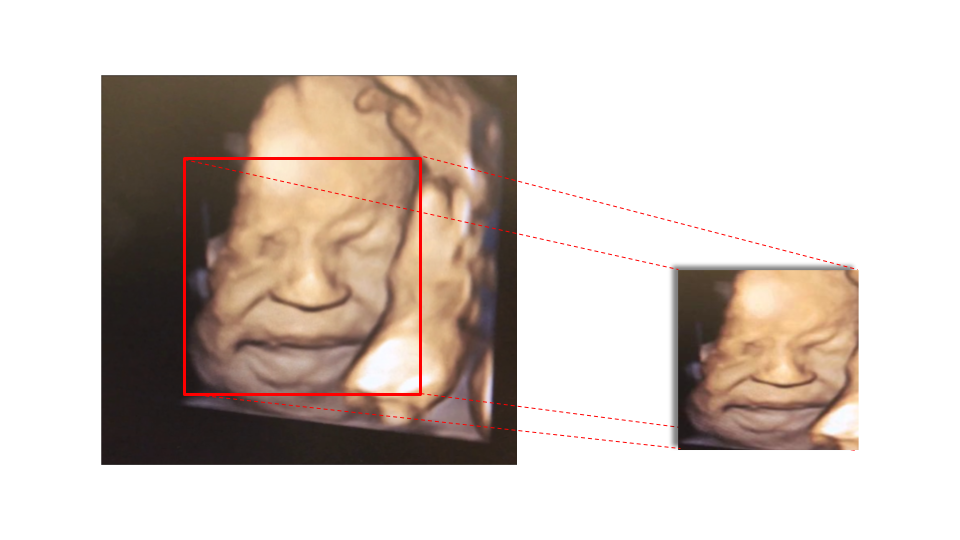
\includegraphics[width=.7\textwidth]{imgs/chap5_cropping.png}
    \caption{Image cropping with MTCNN}
    \label{fig:cropping}
\end{figure}

In the videos of acute pain, as we knew precisely when the anesthetic puncture stimuli were applied, it was possible to divide the images into the two classes of pain and non-pain. This division is relevant, as it allows us to experiment in the scenario where we can evaluate the same fetus, for both conditions. In the other two groups, this is not possible as we have only images of the non-pain class.

\section{Data Augmentation}

Even though we had increased the size of the dataset by turning the videos into images, it is still considered a relatively small dataset for deep learning models. To further augment our chances of succeeding, we have applied the use of data augmentation techniques to increase the variability of our data. The effectiveness of this technique has been demonstrated by \cite{abs-1712-04621} and is widely used in the field.

There is a wide variety of transformations possible for using data augmentation, and even simple techniques already work very well. We have chosen to apply the following transformations:

\begin{itemize}
    \item Horizontal flip, which mirrors the image horizontally. 
    \item Rotation, which applies rotations to the images up to a maximum degree.
    \item Zooming, which zooms into parts of the image up to a maximum level.
    \item Warping, which adds distortions to the image up to a maximum level.
    \item Lighting, which changes the brightness and the contrast of the images.
\end{itemize}

All of these methods have a probability of being applied and can be used in combination with each other. Thus for each image, given the probability, a combination of these techniques would be applied. Some examples of these different combinations within the same image are shown in Figure \ref{fig:data_augmentation}.

\begin{figure}[h!tp]
    \centering
    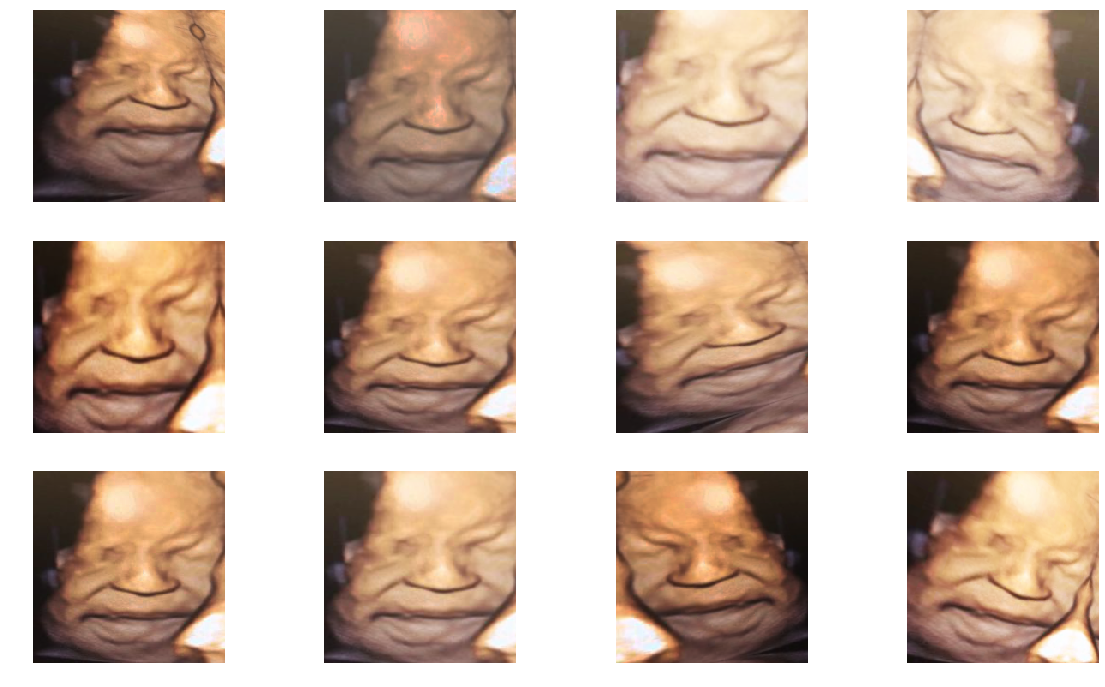
\includegraphics[width=.75\textwidth]{imgs/chap5_data_augmentation.png}
    \caption{Application of different data transformations to a fetus image}
    \label{fig:data_augmentation}
\end{figure}

To further experiment with this process, we have compared two levels of intensity in the changes regarding their max levels of rotation, zoom, warping, and lightning. First, a weak set of transformations, which does subtle changes in the images. Later, a stronger set, which applies substantial changes to the images.

\section{Residual Networks (ResNets)}

Uncountable convolutional neural network architectures have been developed by researchers around the world with many creative modifications, designed for a range of applications. One type of network that is commonly used is the Deep Residual Network (ResNet) developed by \cite{ParkhiVZ15}. This network was the winner of the ImageNet Large Scale Visual Recognition Challenge (ILSVRC) \citep{ILSVRC15}, achieving an error rate of only 3.57\% in the image classification task.

The intuition behind ResNet emerged when the researchers behind the project noticed that as they increased the depth of a regular network, its training and test errors got worse than when compared to an equivalent shallow network. This happens because of a well-known problem, the vanishing gradient. As the gradient back-propagates to the earlier layers of a network, the repeated multiplications make the gradient infinitely small, which prevents it from reaching the weights of the earlier layers.

Other techniques have been developed to deal with this problem, such as batch normalization, but despite that, deeper networks still suffer from degradation in convergence, as the errors remain higher than if it was on an equivalent shallow network.

The insight the authors had, was that when adding extra layers, if these layers are identity mappings, they become equivalent to the shallower network. Thus, the deeper network should not produce an error higher than its shallower counterpart. They achieved this behavior by injecting these identity mappings in the network trough shortcut connections, which are simply connections skipping one or more layers. The output of these layers is added to the outputs of the stacked layers, and add no extra parameter nor computational complexity to the networks.

Another insight they had was regarding residuals, which are just the error in a result. Thus, the network should be able to learn these residuals so that the predictions are closer to the actual values. By combining these two ideas, they have created the residual learning building block, as shown in Figure \ref{fig:building_block} extracted from the original paper.

\begin{figure}[h!tp]
    \centering
    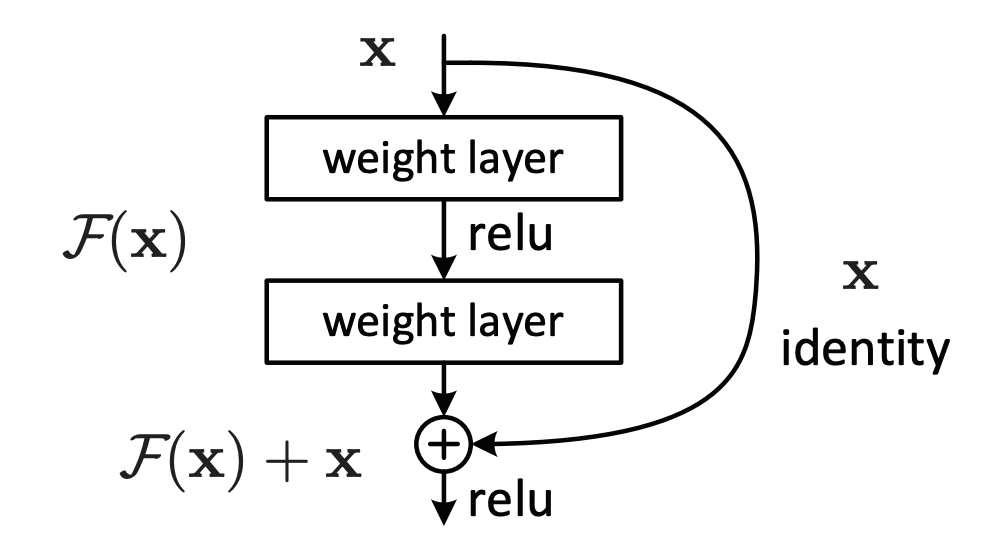
\includegraphics[width=.5\textwidth]{imgs/chap5_building_block.png}
    \caption[Residual Network building block.]{Residual Network building block. Image extracted from \cite{ParkhiVZ15}}
    \label{fig:building_block}
\end{figure}

During the training period, the ResNet learns the weights of its layers in a way that if the identity mapping were optimal, all the weights would be set to zero.

In the diagram, we can see that if $F(x)$ becomes zero, it means $x$ is getting directly mapped to the actual value, and no corrections need to be made. These are the identity mappings that help the network grow deeper. On the other hand, if there is a deviation from optimal identity mapping i.e., a residual, the weights and biases of $F(x)$ will be learned to adjust for it. In other words, $F(x)$ learns how to adjust our predictions to match the actual values.

These building blocks are stacked together to arrive at a deep network architecture. Figure \ref{fig:resnet}, also extracted from the original paper, shows a comparison between a 34-layer plain network and 34-layer ResNet. In our work, we have used 50-layer one with the intuition that a relatively larger network would yield better results.

\begin{figure}[h!tp]
    \centering
    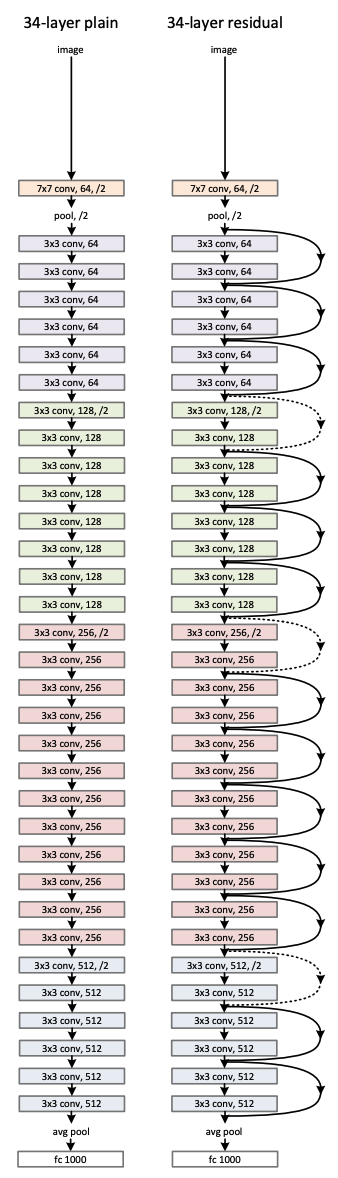
\includegraphics[width=.4\textwidth]{imgs/chap5_resnet.png}
    \caption[34-layer plain network in comparison with 34-layer residual network.]{34-layer plain network in comparison with 34-layer residual network. Image extracted from \cite{ParkhiVZ15}}
    \label{fig:resnet}
\end{figure}

\section{Transfer Learning}

As described in Chapter 3, training a deep neural network from scratch is a very costly task, both in terms of the amount of data necessary as well as in terms of computational power. Because of these factors, transfer learning is often used in a variety of applications as a solution for when we have a limited amount of data, which is especially the case in the medical field. The intuition is that by using pre-trained weights, we can get the benefits of networks trained on much larger datasets, often with millions of images. Then, by changing only the last fully connected layer of the network to match the number of classes in our problem, we are able to fine-tune them with our data.

One general-purpose dataset very often used for pre-training is ImageNet \footnote{\url{http://www.image-net.org}} \citep{DengDSLL009}, which consists of more than 14 million images, which have been hand-annotated by the project to indicate what objects are pictured on them. This visual database was designed for use in visual object recognition software studies and had a significant impact on deep learning research. The most popular network architectures we now today, have emerged in the ImageNet Large Scale Visual Recognition Challenge (ILSVRC), an annual computer vision contest held between 2010 and 2017, which uses a subset of the ImageNet database with 1.2 million images and 1000 classes. 

Convolutional neural networks are very often pre-trained on this dataset, as it contains images of many different categories, like plants, animals, cars, objects, and many others. Hence, by training on this data, the network can learn low-level features such as lines, edges, and basic shapes, but also mid-level features which build on top of the low-level ones, and can detect objects or more complex shapes. These types of features can be considered independent from the final task to some extent, as for many applications detecting basic shapes will often be necessary.

Another popular large-scale dataset used for pre-training is the VGGFace2 \footnote{\url{http://www.robots.ox.ac.uk/~vgg/data/vgg_face2}} \citep{Cao2018}, which consists of 3.3 million images of faces downloaded from Google Image Search, with variations in pose, age, illumination, ethnicity, and profession. A few example images from this dataset can be seen in Figure \ref{fig:vggface}.

\begin{figure}[h!tp]
    \centering
    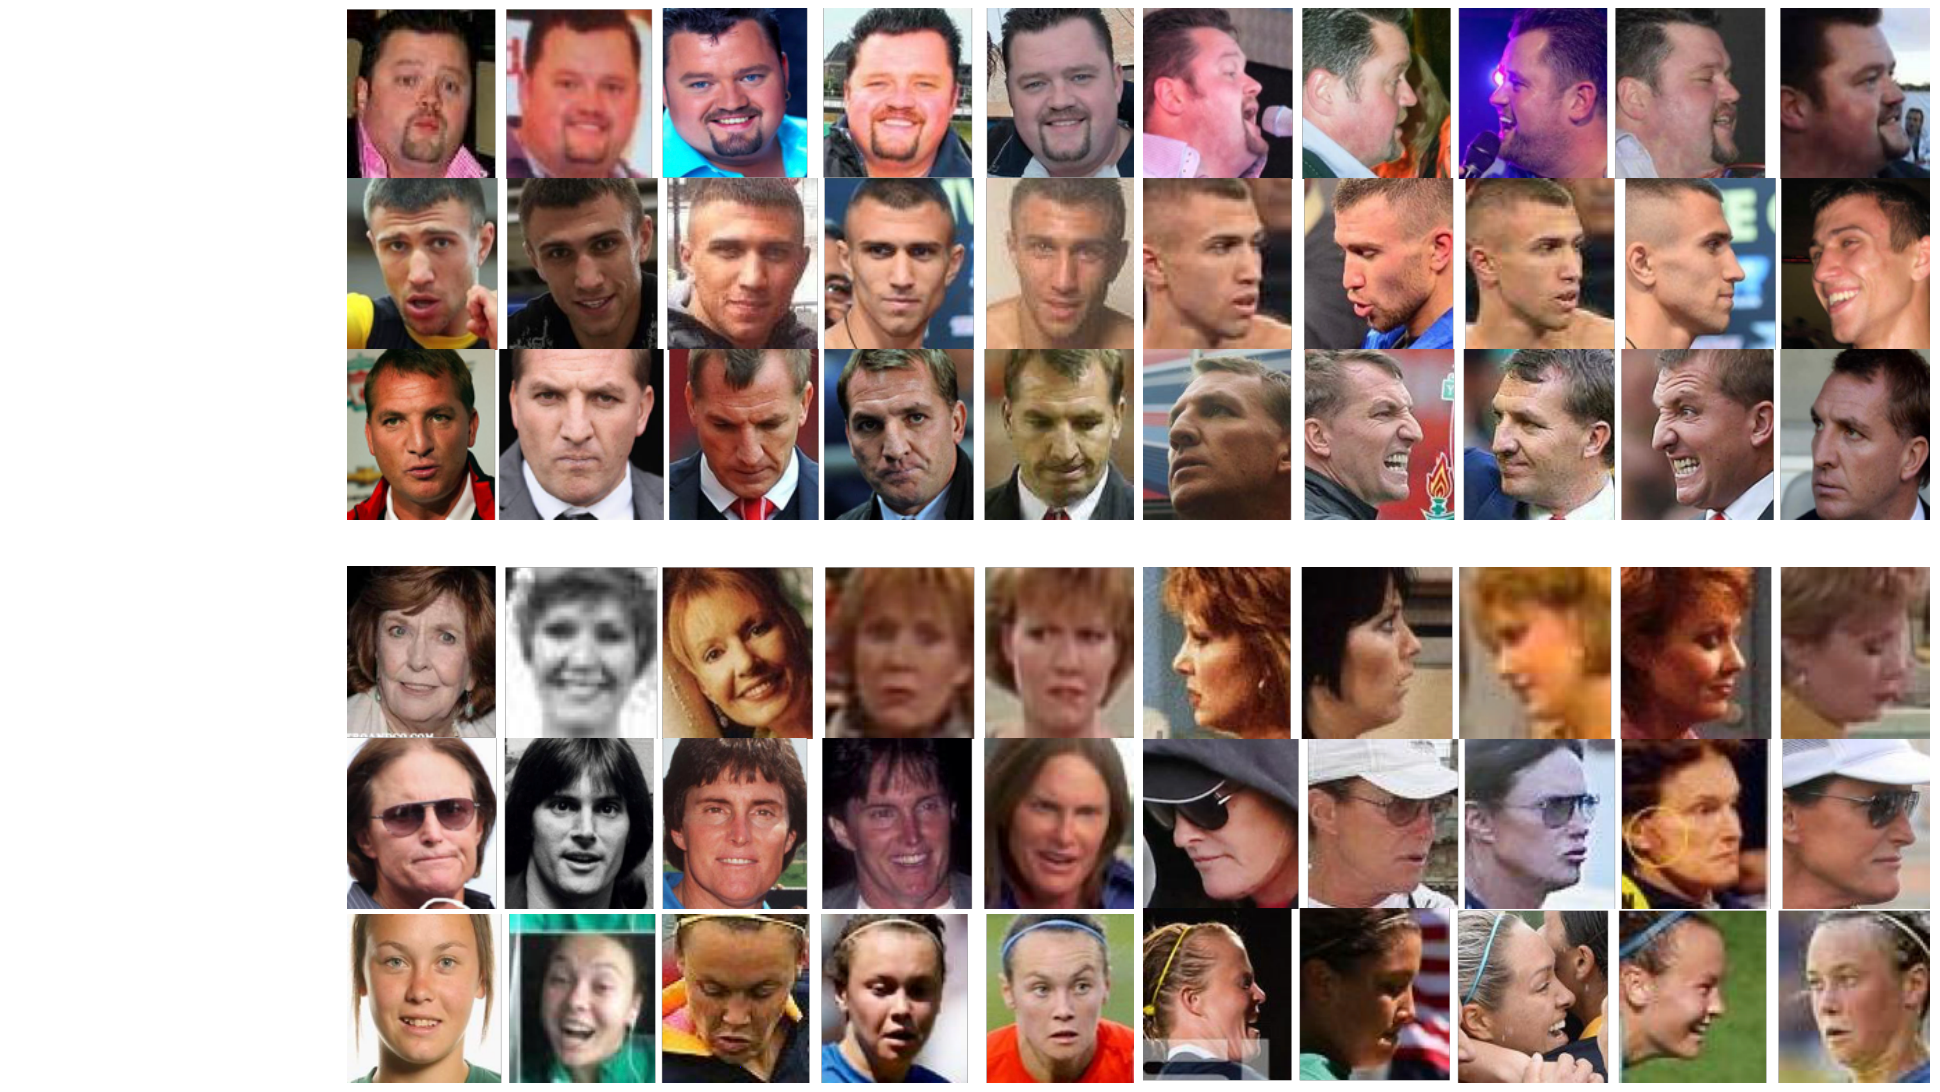
\includegraphics[width=.8\textwidth]{imgs/chap5_vggface2.png}
    \caption[VGGFace2 example images.]{VGGFace2 example images. Images extracted from \cite{Cao2018}}
    \label{fig:vggface}
\end{figure}

This dataset was the same used by \cite{abs-1807-01631} for automatically detecting pain in infants, therefore we hypothesize it would perform well in our data too. We believe the high-level features learned by a network trained on this dataset should be able to detect similar features to the ones we aim to detect in fetuses, such as the mouth, the nose, and the eyes, to mention a few.

\subsection{Fine-tuning}

When using transfer learning, the features computed in the early layers of the network usually are already well trained in doing basic tasks such as recognizing basic lines, patterns, or gradients. On the other hand, the features computed in the later layers are the ones highly dependent on the specific task we are trying to predict. Thus, when we are fine-tuning the network in our domain, we have two main approaches to train the network, namely with frozen or unfrozen layers. These methods allow us to decide which specific layers of our model we want to train at a given time. 

In the frozen approach, all layers except the last one will not be trainable. In the unfrozen approach, however, all the layers are kept unfrozen during training, and the errors are back-propagated to the entire network during fine-tuning. Hence, even the early layers may be affected. In our experiments, we decided to test both approaches, as even though unfreezing the layers appears to be better, we were unsure if the amount of data and its noise would be enough to improve the weights of the whole network.




